\documentclass[12pt]{article}
\usepackage{graphicx} % Required for inserting images
\usepackage{geometry}
\usepackage{amsmath}
\usepackage{amsfonts}
\usepackage{amssymb}
\usepackage{float}
\usepackage[spanish]{babel}
\usepackage[utf8]{inputenc}
\usepackage{textcomp}
\usepackage{xcolor} % Use xcolor instead of color for more options, including 'gray'
\usepackage{setspace}
\usepackage{pdfpages}
% Add references
\usepackage{cite}
\usepackage{hyperref}
\usepackage{listings} % Required for code listings

\hypersetup{
    colorlinks=true,
    linkcolor=black,    % Keep internal links black (or change to oro)
    citecolor=black,    % Keep citation links black (or change to oro)
    filecolor=black,    % Keep file links black (or change to oro)
    urlcolor=oro,       % Use your defined 'oro' color for URLs
    pdftitle={Práctica Spark},
    pdfpagemode=FullScreen,
}
\definecolor{oro}{rgb}{0.83, 0.69, 0.22}
\geometry{left=2.54cm,top=2.54cm,right=2.54cm,bottom=2.54cm}

% Define Python code style for listings
\lstdefinestyle{python}{
    language=Python,
    basicstyle=\ttfamily\small,
    keywordstyle=\color{blue},
    stringstyle=\color{red},
    commentstyle=\color{green},
    morecomment=[l]{\#},
    showstringspaces=false,
    breaklines=true,
    frame=single, % Add frame around code
    numbers=left, % Add line numbers
    numberstyle=\tiny\color{gray}
}


\begin{document}

\begin{titlepage}
\begin{center}
{\huge \textbf{Universidad Nacional Aut\'onoma de M\'exico}}\\
\vspace{3mm}
{\LARGE {Por mi raza hablará el espíritu''}}\\
\vspace{3mm}
\begin{figure}[H] % Use H for exact placement if needed, otherwise [h]
\centering
% Consider using a relative path or placing UNAM.pdf in the same directory
\includegraphics[scale=1]{C:/Users/Jorge/Documents/Escolar/UNAM.pdf} % Assuming UNAM.pdf is in the same directory or a standard graphics path
\end{figure}
{\LARGE \textbf{Facultad de Estudios Superiores Acatlán}}\\
\vspace{3mm}
{\LARGE Licenciatura en Matemáticas Aplicadas y Computación}\\
\vspace{5mm}
\textcolor{oro}{\rule{\linewidth}{1mm}}\\
\vspace{2mm}
\begin{spacing}{1.5}
{\LARGE \textsc{Práctica Spark}} %Título del trabajo
\end{spacing}
\textcolor{oro}{\rule{\linewidth}{1mm}}\\
\vspace{1cm}
{\LARGE \textbf{Programación Paralela y Concurrente}}\\ %Nombre de la materia
\vspace{5mm}
\vspace{4mm}
{\LARGE {Peralta Cortés Jorge Alejandro}}\\ %Nombre del alumno
\vspace{4mm}
\vspace{4mm}
\vspace{1cm}
{\LARGE {Doctor José Gustavo Fuentes Cabrera}}\\ %Nombre del profesor
\end{center}
\vfill % Pushes the date to the bottom
\end{titlepage}

\newpage

\section{Introducción}
    Esta práctica consiste en la aplicación de Apache Spark para analizar el tráfico en el sistema de bicicletas públicas Ecobici de la Ciudad de México. El objetivo es procesar un gran volumen de datos de viajes para extraer información útil sobre el uso del sistema, como las estaciones más populares y las horas pico de actividad. Spark es una herramienta ideal para este tipo de tareas debido a su capacidad para procesar grandes conjuntos de datos de manera distribuida y eficiente.

\section{Descripción de los datos}
    Los datos utilizados en este análisis provienen del portal de datos abiertos del sistema Ecobici de la Ciudad de México (\href{https://ecobici.cdmx.gob.mx/datos-abiertos/}{Ecobici Datos Abiertos}). Se descargaron los archivos históricos mensuales en formato CSV, cubriendo el período desde abril de 2024 hasta marzo de 2025.
    Estos datos están organizados principalmente en dos tipos de archivos:
    \begin{itemize}
        \item \textbf{Historial de Viajes:} Archivos CSV mensuales que contienen detalles sobre cada viaje realizado.
        \item \textbf{Ubicación de Cicloestaciones:} Un archivo CSV que contiene información sobre cada estación de Ecobici, incluyendo su ubicación geográfica.
    \end{itemize}

    A continuación, se describen las columnas más relevantes utilizadas en el análisis:

    \begin{description}
        \item[\texttt{df (Viajes)}] - Dataframe que contiene la información unificada de todos los viajes mensuales.
        \begin{itemize}
            \item \texttt{Genero\_Usuario}: Género registrado del usuario ('M', 'F', 'O').
            \item \texttt{Edad\_Usuario}: Edad registrada del usuario.
            \item \texttt{Bici}: Identificador único de la bicicleta utilizada.
            \item \texttt{Ciclo\_Estacion\_Retiro}: ID numérico de la cicloestación donde se retiró la bicicleta.
            \item \texttt{Fecha\_Retiro}: Fecha en que se retiró la bicicleta (YYYY-MM-DD).
            \item \texttt{Hora\_Retiro}: Hora en que se retiró la bicicleta (HH:MM:SS).
            \item \texttt{Ciclo\_EstacionArribo}: ID numérico de la cicloestación donde se devolvió la bicicleta.
            \item \texttt{Fecha\_Arribo}: Fecha en que se devolvió la bicicleta (YYYY-MM-DD).
            \item \texttt{Hora\_Arribo}: Hora en que se devolvió la bicicleta (HH:MM:SS).
        \end{itemize}
        \item[\texttt{df\_stations (Estaciones)}] - Dataframe que contiene la información de las cicloestaciones.
        \begin{itemize}
            \item \texttt{num\_cicloe}: Identificador numérico único de la cicloestación. Usado como clave para unir con los datos de viajes.
            \item \texttt{calle\_prin}: Nombre de la calle principal donde se ubica la estación. Usado para identificar las estaciones en los resultados.
            \item \texttt{latitud}: Latitud geográfica de la estación. Usada para visualización en mapas.
            \item \texttt{longitud}: Longitud geográfica de la estación. Usada para visualización en mapas.
        \end{itemize}
    \end{description}

\section{Tratamiento y Operaciones con Spark}
    El procesamiento de los datos se realizó utilizando Spark, con su API de Python PySpark. Las operaciones clave fueron las siguientes:

    Dado que los datos históricos de viajes estaban divididos en archivos CSV mensuales, el primer paso fue cargarlos y unificarlos en un único DataFrame Spark.
    \begin{itemize}
        \item Cada archivo CSV fue leído en un DataFrame Spark usando \texttt{spark.read.csv}
        \item Los nombres de las columnas que contenían espacios fueron renombrados reemplazando los espacios por guiones bajos para facilitar su manejo en Spark SQL y operaciones de DataFrame.
        \item Todos los DataFrames individuales fueron combinados en uno solo usando la operación \texttt{union}. Esto con el propósito de tener un dataset con una gran cantidad de datos para probar las capacidades de Spark.
    \end{itemize}

    \begin{lstlisting}[style=python, caption={Carga y unificación de archivos CSV mensuales.}, label={lst:load_data}]

path = 'Datos/Historicos/*.csv'
files = glob.glob(path)

dfs = []
for file in files:

temp_df = spark.read.csv(file, header=True, inferSchema=True)
    temp_df = temp_df.toDF(*[col.replace(' ', '_') for col in temp_df.columns])
    print(f"Loaded {file} with {temp_df.count()} rows")
    dfs.append(temp_df)

# Unificar todos los dataframes en uno solo
df = dfs[0]
for i in range(1, len(dfs)):
    df = df.union(dfs[i])

df.printSchema()
    \end{lstlisting}

    Para determinar las estaciones más populares, se agruparon los datos de viajes por estación de retiro y arribo usando \texttt{groupBy}. Esto permitió contar el número de viajes iniciados y finalizados en cada estación. Las columnas \texttt{Ciclo\_Estacion\_Retiro} y \texttt{Ciclo\_EstacionArribo} fueron utilizadas como claves para estas agrupaciones.

    Para añadir información geográfica (latitud, longitud) y el nombre de la calle a las cuentas de retiros y arribos, se realizó una unión (join) con el DataFrame de estaciones (\texttt{df\_stations}).
    \begin{itemize}
        \item Se utilizó \texttt{join} para combinar las cuentas de retiros (\texttt{station\_departure\_counts}) con la información de las estaciones (\texttt{stations\_info}) usando \texttt{station\_id} como clave. Se usó un \texttt{left join} para mantener todas las estaciones que tuvieron retiros.
        \item Se realizó otro \texttt{left join} para añadir las cuentas de arribos (\texttt{station\_arrival\_counts}) al resultado anterior, nuevamente usando \texttt{station\_id} como clave.
    \end{itemize}

    \begin{lstlisting}[style=python, caption={Cálculo de viajes por estación y unión con información geográfica.}, label={lst:join_stations}]
station_departure_counts = df.groupBy('Ciclo_Estacion_Retiro') \
                             .count() \
                             .withColumnRenamed('Ciclo_Estacion_Retiro', 'station_id') \
                             .withColumnRenamed('count', 'count_retiro')

station_arrival_counts = df.groupBy('Ciclo_EstacionArribo') \
                           .count() \
                           .withColumnRenamed('Ciclo_EstacionArribo', 'station_id') \
                           .withColumnRenamed('count', 'count_arribo')

stations_info = df_stations.select(
    F.col('num_cicloe').alias('station_id'),
    F.col('calle_prin').alias('station_name'),
    'latitud',
    'longitud'
)

station_counts_with_info = station_departure_counts.join(
    stations_info,
    on='station_id',
    how='left'
)

station_count_clean = station_counts_with_info.join(
    station_arrival_counts,
    on='station_id',
    how='left'
)

station_count = station_count_clean.fillna(0, subset=['count_retiro', 'count_arribo'])

station_count.orderBy('count_retiro', ascending=False).show(10)
    \end{lstlisting}

    Para identificar las horas pico de uso, se extrajo la hora del día de las columnas \texttt{Hora\_Retiro} y \texttt{Hora\_Arribo}.
    \begin{itemize}
        \item Se aplicó \texttt{groupBy} sobre la columna de hora extraída (\texttt{hora\_retiro} o \texttt{hora\_arribo}) seguido de \texttt{count()} para obtener el número de viajes por cada hora del día.
        \item Los resultados se ordenaron para ver las horas con mayor tráfico.
    \end{itemize}

    \begin{lstlisting}[style=python, caption={Extracción y conteo de viajes por hora de retiro.}, label={lst:hourly_traffic}]
df_with_hour = df.withColumn("hora_retiro", F.hour(F.to_timestamp(F.col("Hora_Retiro"), "HH:mm:ss")))

hourly_traffic = df_with_hour.groupBy("hora_retiro").count().orderBy("count", ascending=False)

print("Horas de mayor retiro:")
hourly_traffic.show()
    \end{lstlisting}

    Se utilizaron las bibliotecas \texttt{Plotly Express} y \texttt{Pandas} para visualizar los resultados. Los DataFrames de Spark con los resultados agregados (conteos por estación, tráfico por hora) se convirtieron a DataFrames de Pandas usando \texttt{.toPandas()}. \textbf{Nota:} Esta operación recolecta todos los datos en el nodo driver y debe usarse con precaución en conjuntos de datos muy grandes. Para incluir las gráficas en este reporte, fueron guardadas como archivos de imagen (e.g., PNG) desde el notebook.
    \begin{itemize}
        \item Se generaron mapas de dispersión geográficos (\texttt{px.scatter\_mapbox}) para mostrar la ubicación de las estaciones, con el tamaño y color de los puntos representando la cantidad de retiros o arribos.
        \item Se crearon gráficos de barras (\texttt{px.bar}) para visualizar la distribución del tráfico a lo largo de las horas del día.
    \end{itemize}

\section{Análisis de los Resultados}
    El análisis de los datos procesados con Spark reveló varios patrones interesantes sobre el uso de Ecobici:

    \begin{itemize}
        \item \textbf{Estaciones Populares:} Al observar los resultados de \texttt{station\_count.orderBy('count\_retiro', ascending=False).show(10)} y \texttt{station\_count.orderBy('count\_arribo', ascending=False).show(10)}, se identificaron las 10 estaciones con mayor número de retiros y arribos, respectivamente. Estas estaciones suelen concentrarse en zonas de alta densidad poblacional, centros de trabajo u oficinas, y puntos de conexión con otros sistemas de transporte. La visualización en el mapa (Figura \ref{fig:mapa_retiros} y \ref{fig:mapa_arribos}) confirma esta concentración geográfica.
        \item \textbf{Horas Pico:} El análisis del tráfico por hora (\texttt{hourly\_traffic.show()}) mostró picos claros de actividad.
            \begin{itemize}
                \item \textbf{Retiros:} Se observó un pico importante en las mañanas (típicamente entre 7-9 AM) y otro aún mayor en las tardes (alrededor de 5-7 PM). Esto sugiere un uso predominante para traslados hacia y desde el trabajo o estudio (ver Figura \ref{fig:hora_retiros}).
                \item \textbf{Arribos:} Los picos de arribos siguen una lógica similar pero ligeramente desfasada, con un pico por la mañana (llegadas al destino) y un pico más pronunciado por la tarde/noche (regresos a casa o puntos de origen) (ver Figura \ref{fig:hora_arribos}).
            \end{itemize}
            Los gráficos de barras generados con Plotly visualizaron claramente estas tendencias horarias.
        \item \textbf{Distribución Geográfica:} Los mapas interactivos (Figuras \ref{fig:mapa_retiros} y \ref{fig:mapa_arribos}) mostraron que la actividad de Ecobici no es uniforme en toda la red. Hay "hotspots" claros donde la demanda (retiros) y la oferta (arribos) son significativamente más altas. Comparar los mapas de retiros y arribos puede indicar desbalances (estaciones donde se acumulan o faltan bicicletas en ciertos horarios).
    \end{itemize}

    \subsection{Visualizaciones}

    \begin{figure}[htbp]
        \centering
        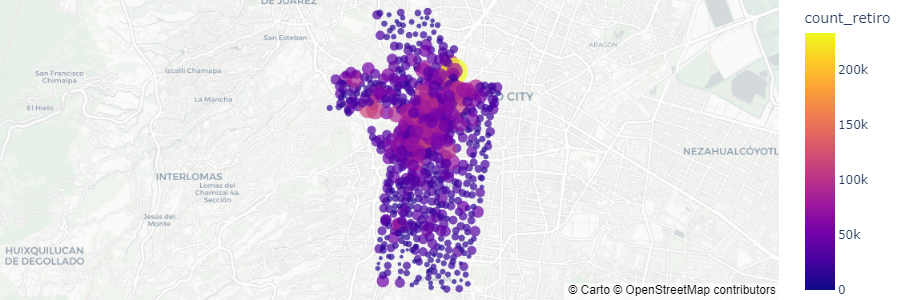
\includegraphics[width=0.9\textwidth]{Media/mapa_retiro.png} % Reemplaza con tu nombre de archivo
        \caption{Mapa de calor de retiros por estación. El tamaño y color indican mayor número de retiros.}
        \label{fig:mapa_retiros}
    \end{figure}

    \begin{figure}[htbp]
        \centering
        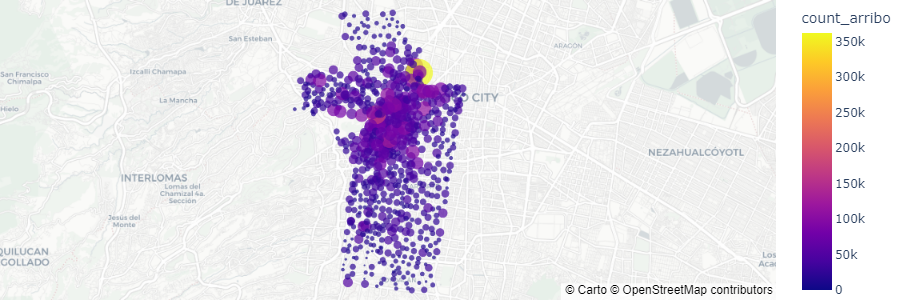
\includegraphics[width=0.9\textwidth]{Media/mapa_arribo.png} % Reemplaza con tu nombre de archivo
        \caption{Mapa de calor de arribos por estación. El tamaño y color indican mayor número de arribos.}
        \label{fig:mapa_arribos}
    \end{figure}

    \begin{figure}[htbp]
        \centering
        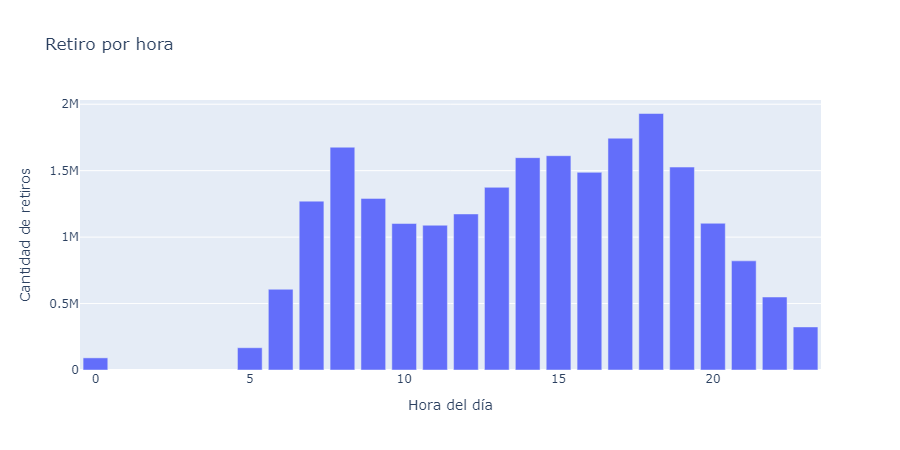
\includegraphics[width=0.8\textwidth]{Media/retiros_hora.png} % Reemplaza con tu nombre de archivo
        \caption{Número total de retiros por hora del día.}
        \label{fig:hora_retiros}
    \end{figure}

    \begin{figure}[htbp]
        \centering
        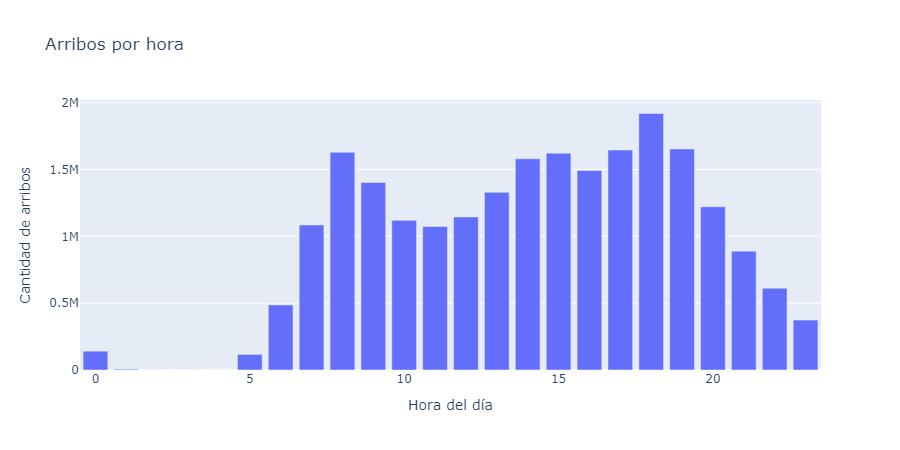
\includegraphics[width=0.8\textwidth]{Media/arribos_hora.png} % Reemplaza con tu nombre de archivo
        \caption{Número total de arribos por hora del día.}
        \label{fig:hora_arribos}
    \end{figure}

    \clearpage % Asegura que las figuras no se solapen con la siguiente sección

\section{Reflexión sobre el uso de Spark}
    Spark está diseñado para el procesamiento distribuido, y muchas de las operaciones realizadas en este análisis se benefician enormemente de esta capacidad:

    \begin{itemize}
        \item \textbf{Operaciones Eficientemente Distribuibles:}
            \begin{itemize}
                \item \textbf{Transformaciones por Fila (\texttt{withColumn}, \texttt{toDF}, \texttt{select}):} Operaciones como renombrar columnas, extraer la hora (\texttt{hour(to\_timestamp(...))}), o seleccionar columnas se aplican a cada partición de datos de forma independiente y paralela.
                \item \textbf{Agregaciones (\texttt{groupBy().count()}):} Estas operaciones son altamente paralelizadas en Spark. Lo que permite tener mejor rendimiento que en pandas.
                \item \textbf{Uniones (\texttt{join}):} Spark puede realizar la unión de manera distribuida, lo que significa que puede combinar grandes conjuntos de datos sin pasar por un único núcleo o dispositivo.
            \end{itemize}
        \item \textbf{Operaciones Menos Distribuibles o Potenciales Cuellos de Botella:}
            \begin{itemize}
                \item \textbf{\texttt{.toPandas()}:} Esta operación recolecta \textit{todos} los datos del DataFrame  para crear un DataFrame de Pandas en la memoria. Si el DataFrame resultante es muy grande, puede causar errores de memoria o ser extremadamente lento. Es útil para visualización o integración con bibliotecas que no son de Spark.
                \item \textbf{Lectura de Muchos Archivos Pequeños:} Si bien Spark puede leer múltiples archivos, leer una cantidad masiva de archivos muy pequeños puede ser ineficiente debido a la sobrecarga de iniciar una tarea por cada archivo. En tales casos, sería mejor consolidar los archivos pequeños primero. En este caso, con archivos mensuales, la sobrecarga es probablemente manejable.
            \end{itemize}
    \end{itemize}
\section{Uso de IA}
    En esta práctica, se utilizó IA para generar el texto del reporte y las visualizaciones. La IA ayudó a resumir los resultados.
    Asimismo, se utilizó IA principalmente para encontrar las equivalencias entre las funciones de pandas y las de Spark, aunque al final no fue tan necesario, ya que la mayoría de funciones son muy similares
    El código generado se puede consultar en el siguiente repositorio de GitHub: \href{https://github.com/Jorge95Cortes/Spark-practice.git}{Spark-practice}.
\end{document}